\documentclass[12pt]{article}
\setlength{\oddsidemargin}{0in}
\setlength{\evensidemargin}{0in}
\setlength{\textwidth}{6.5in}
\setlength{\parindent}{0cm}
\setlength{\parskip}{\baselineskip}


\usepackage{amsmath,amsfonts,amssymb,amsthm,graphicx}
\usepackage{hyperref}

\graphicspath{{./images/} }
\title{\vspace{-7ex}Topological Features of Go Games \vspace{-2ex}}
\author{Edward Kim}
\date{\vspace{-2ex}\today}
\begin{document}
\maketitle

\section{Introduction}
Go, Weiqi, or Baduk is an abstract strategy game where two players compete to enclose and control as much territory as possible on the board. Stones are placed on a board typically consisting of nineteen parallel vertical lines and  nineteen parallel horizontal lines; the stones are placed on the intersections. Players create chains of stones that act as a wall demarcating territory and invade each other's territory both to reduce their opponent's territory and to cement their own. The game's strategic complexity arises from the web of dependencies which appear to be local in scope but global in influence. The centuries of game records and pattern research alone bespeaks of the its hidden labyrinth of complexity.

The difficulty of analyzing the game's strategic dynamics is further evident in the hoary line of trial-and-error pursuits that is Go AI research. As mentioned in the proposal, Go AI have only recently achieved the level of professional play. While Chess AI have performed at professional levels, Go AI have historically only performed at the level of a weak amateaur \cite{bays},\cite{muller}. In addition to the massive search space, many of the moves are deemed illegal. M{\" u}ller  makes the explicit point that only about 1.2\% of all $3^{19 \times 19}$ board configurations are legal configurations \cite{muller}. This puts even more computational strain on an already gargantuan search space. The infeasiblability of creating a half-decent evaluation function to determine the strategic value of any move further compounds the challenge of creating a competent computer player.

However, the seminal victory of the AI player, AlphaGo against 9-dan professional, Lee Sedol became a startling yet monumentous achievement in AI history. Through the techniques of reinforcement learning and Monte-Carlo Tree Search, Google Deepmind was able to create a formidable player which won four out of five matches against Lee Sedol. \cite{alpha} A more recent iteration, AlphaGo Zero, has recently shown even stronger play. The plays from both AI players will be considered in this report.

As mentioned in the proposal, the promise behind using persistent homology on Go games derives from the inherent nature of the patterns arising from the game. Go players frequently create local patterns which are yet part of a set of global patterns on the board \cite{bays}. Tracking these local patterns as the scope becomes broader was one of the major goals pursued by this project. The following revised questions guided the direction of this project:
\begin{itemize}
  \item Can we track the connectivity strength between stone groups changes as the game progresses?
  \item How are games between experienced and inexperienced players different topologically?
  \item Can we determine advantage differentials? As in, can we determine if one player is clearly winning over the other? In particular, do games played by AI exhibit different traits than games played by humans?
\end{itemize}

This report will elaborate on the small successes revealed through TDA techniques and the hurdles which currently preclude deeper analysis of Go games beyond traits seen in the most global scope. All of of the relevant definitions will be explained in the paper as needed.

\section{Basic notions}

As mentioned in the introduction, players place stones of their own color on the intersections of board consisting of nineteen parallel vertical lines and nineteen parallel horizontal lines. Players alternate turns but have the option to forgo their turn. If both players pass, the game ends and the scoring phase commences.

A player's stones are captured if the opponent's stones occupy all adjacent horizontal and vertical intersections. Accordingly, empty adjacent horizontal and vertical intersections are called \textit{liberties}. See Figure \ref{fig:lib1} for an example.
\begin{figure}[ht]
  \centering
  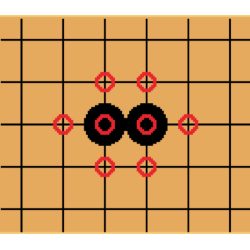
\includegraphics{lib1.png}
  \caption{A simple example of a pair of black stones and its liberties}
  \label{fig:lib1}
\end{figure}

A stones can form extended chains or groups which serve to demarcate territory.


\section{Analysis Engine and Data Sources}

To facilitate proper formulation of ideas for analysis and visualization of persistence diagrams, we developed an extensive analysis engine, TDAGo \cite{tdago}. TDAGo was developed in Python 3 with following libraries:
\begin{itemize}
   \item sgfmill, a SGF game format parsing library
   \item risper and persim, persistent homology libraries
   \item matplotlib, a data plotting library
\end{itemize}

The analysis engine parses the sgf formats and pipes the data into ripser to generate persistence diagrams. It supports a variety of modes including animating the progression of the persistence diagrams for each color as the game progresses. All experiments and persistence diagram plots were created through this engine. The github repository is licensed under the MIT license and is considered open-source. All plots used in this report will be archived in the TDAGo repository.

We use primary use data sources from FoxGoDB \cite{fox} and publicly available AlphaGo archives \cite{alphalib}. All games are transcribed into the universal SGF format for simple retrival.

\section{Basic observations}

We begin with some immediate observations concerning persistence diagrams corresponding to board states. We will reference Figure \ref{fig:lsd1} as needed.
\begin{figure}[ht]
  \centering
  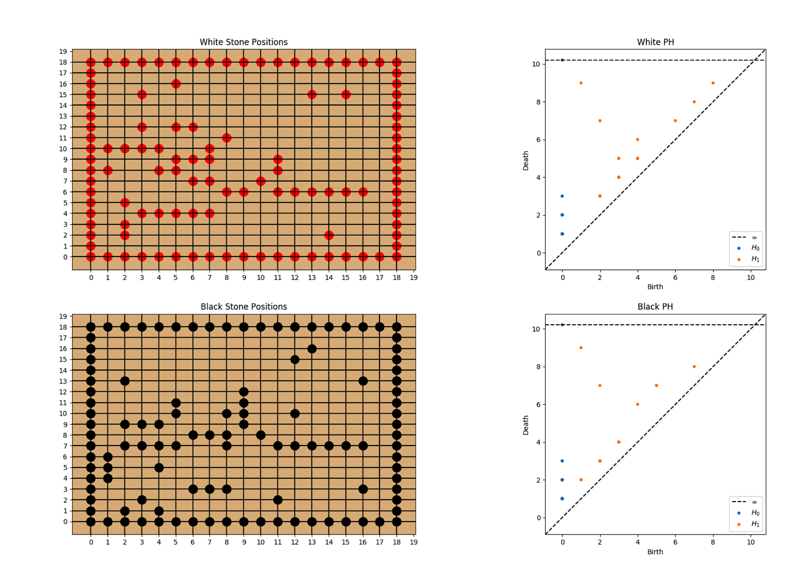
\includegraphics{lsd1.png}
  \caption{The persistence diagrams for the black and white board state for Lee Sedol vs AlphaGo Master: Move 82}
  \label{fig:lsd1}
\end{figure}

Since all adjacent points of intersection on the board are equidistant from one another, every stone's coordinates be a pair of nonnegative integers. Consequently, the birth and death times will both be nonnegative integers as well. We compute our persistence homology cycles by running the library ripser with the Manhatten metric. This metric between two stones has the natural interpretation as the number of subsequent moves a player must make to connect the pair of stones. By observing the behavior of the persistence diagrams as the gane progresses for both players, we come to the following interpretation for the birth and death times:
\begin{itemize}
  \item From the construction of the Vietoris-Rips complex, we can deduce that the birth times will be upper bounds on the number of stones required to connect a pair of consecutive stones along the \textit{boundary}. In other words, to fully enclose the group detected, the player will expect to spend at most $b\cdot n$ consecutive moves where $n$ is the number of stones contained in the detected chain and $b$ is the birth time of the detected chain.
  \item The death times are interpreted as an upper bound on the number of stones required to connect \textit{any} pair of stones in the chain. Once again from the construction of the Vietoris-Rips complex, we can see that any two stones in the chain can be connected by $2d$ stones where $d$ is the death time of the detected chain. Intuitively, we can think of a higher death time as an indication of a larger enclosed area. However, there are some obstacles to this view as we will see later in the report.
\end{itemize}

From these two interpretations, we can start to valuate chains by placing higher value on chains which have lower birth times and higher death times. Lower birth times signify stronger connectivity between the stones in the chain. Stronger connectivity repels any attempt by the opponent to invade and segment the group. Higher death times indicate broadness or a larger span which the chain potentially controls. We proactively used the connectivity data to gauge both human and machine player performance during this project.

\section{Concerning Connectivity}

As mentioned in the previous section, shorter distances between stones in a chain are desired as such chains are easier to cement into captured territory. For instance, consider the board in Figure \ref{fig:conn1}. Observe the chain of white stones around the center of the board. A cursory glance shows that if the white player desired to complete the chain, he or she will have to spend around three moves to connect one stone of the boundary to the next stone. Compare this to chain of black stones surronding the aforementioned chain of white stones. Due to the glaring lack of stones at far-left side of the board, the black player must invest more moves to fortify the side. Note that since the white player has higher prospects, he can use this weakness to cut the black player's chain in half.
\begin{figure}[ht]
  \centering
  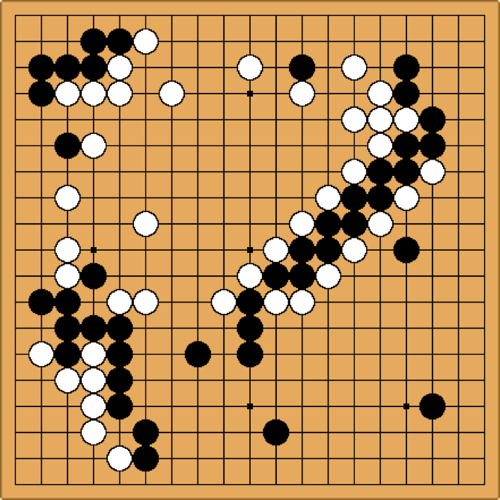
\includegraphics{conn1.png}
  \caption{An example board state illustrating connectivity strength between stones}
  \label{fig:conn1}
\end{figure}

These observations inspired us to use connectivity to predict the victor for games played between players of similar rank. The hope was that connectivity would shed a bit of light on the game dynamics seen in novice play in constrast to the presumably more complicated dynamics seen in professional-level play.

Through TDAGo, we were able to create a simple connectivity graph by taking the birth times seen for say the black player's board state and simply averaging the birth times of all one-dimensional features detected. 





\bibliography{biblo}
\bibliographystyle{ieeetr}

\end{document}
